\subsection{Atmospheric mercury concentration}\label{sec:lidar}

To illustrate how monotonicity changes derivative inference, we use
all $221$ released mercury lidar observations over
$390$--$720$ meters near the Bella Vista geothermal power station in
Italy, distributed with the R package SemiPar
\citep{holst1996lidar,feng2022sshaped}. Each response is the log ratio
of reflected on-resonant and off-resonant laser signals, with
approximately $100$ pulse pairs averaged during acquisition.
These data have also been analyzed with a globally monotone GP
approximation by \citet{maatouk2025bayesian}.

The shape restriction follows from the differential absorption lidar
(DIAL) approximation, which neglects differential backscatter and
attenuation from other species. Under this approximation, the derivative
of the mean log ratio per meter equals mercury concentration multiplied
by $-1.6\times10^{-5}$ square meters per nanogram. Nonnegative
concentration therefore requires a nondecreasing latent mean for the
negative log ratio, even if the noisy observations are not ordered.

Write $r$ for distance in meters, set $x(r)=(r-390)/330$, and let $Y_i$
be the negative recorded log ratio. We use $128$ basis functions with
center $c=1/2$ and half-width $L=2$, so the computational interval
$[-1.5,2.5]$ contains the physical interval $[0,1]$.
The Mat\'{e}rn $7/2$ spectral prior in \cref{eq:finite-model} gives
the hierarchy
\[
\begin{aligned}
 f_{\boldsymbol a}(x)&=a_0+\sum_{j=1}^{128}a_j\phi_{j,2}(x),
 \qquad a_0\sim N(\mu_0,\sigma_0^2),\\
 a_j&\overset{\mathrm{ind}}\sim
 N\left(0,\sigma_f^2\frac{32\lambda^7}{5(\lambda^2+\omega_j^2)^4}\right),
 \qquad \lambda=\frac{\sqrt7}{\ell},\\
 Y_i\mid\boldsymbol a&\overset{\mathrm{ind}}\sim
 N(f_{\boldsymbol a}(x(r_i)),\sigma_i^2).
\end{aligned}
\]
The intercept is independent of the other coefficients, with prior
mean $\mu_0=0.291156$ and standard deviation $\sigma_0=1.952921$.
These values are the observed response mean and twice its range,
respectively. The underlying
GP has marginal standard deviation $\sigma_f=0.308590$ and normalized
length scale $\ell=0.288869$, corresponding to $95.33$ meters.

Following the noise family of \citet{holst1996lidar}, we allow
measurement variance to change with distance by setting
\[
 \sigma_i=\sigma_{\mathrm{mid}}
 \exp\bigl(\gamma_1(x(r_i)-c)+\gamma_2(x(r_i)-c)^2\bigr).
\]
Here $\sigma_{\mathrm{mid}}=0.056125$ is the noise standard deviation
at the midpoint of $555$ meters, while $\gamma_1=2.330252$ and
$\gamma_2=-0.305387$ describe the linear and quadratic changes in
its logarithm. All standard deviations are on the negative-logratio
scale. We estimate the covariance and noise parameters jointly by
ordinary underlying-GP marginal likelihood and use the same estimates
in both posterior fits.

The inferential targets are the latent negative log ratio
$f_{\boldsymbol{a}}(x(r))$ and the implied concentration
\[
 \frac{1}{330(1.6\times10^{-5})}\left.\frac{\mathrm{d}f_{\boldsymbol{a}}}{\mathrm{d}x}\right|_{x=x(r)}
 \quad\text{nanograms per cubic meter}.
\]
The factor $330$ converts the derivative in normalized coordinates to
a derivative per meter, so conditioning on $\frac{\mathrm{d}f_{\boldsymbol{a}}}{\mathrm{d}x}(x)\geq0$
throughout $[0,1]$ imposes nonnegative concentration over
the observed range. We use the procedure in \cref{sec:computation}
for the monotone posterior and evaluate the unconstrained Gaussian
summaries analytically. Sampler settings, convergence diagnostics, and
the full posterior predictive assessment are given in the supplementary
material.

\cref{fig:lidarcurves} compares concentration inference with and without monotonicity under the same Gaussian model.
At $502.86$ meters, the ordinary posterior mean concentration reaches its minimum on the reconstruction grid at $-42.13$ nanograms per cubic meter, with pointwise $95\%$ equal-tail credible interval $(-94.27,10.00)$ and posterior probability $0.9434$ of a negative concentration.
Conditioning on monotonicity gives a mean concentration of $11.75$ nanograms per cubic meter at that distance, with corresponding interval $(1.10,31.23)$, while changing the response fit little.

\begin{figure}[H]
\centering
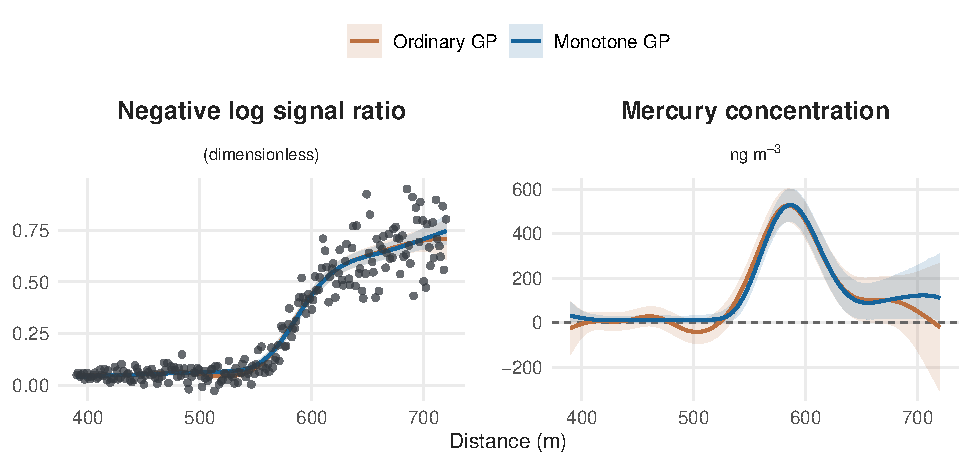
\includegraphics[width=\textwidth]{figures/lidar_monotone_fit.pdf}
\caption[Absorption and concentration inference for mercury lidar]{
The left panel shows the latent negative log signal ratio with all $221$ observations as points, and the right shows mercury concentration in nanograms per cubic meter, given under the DIAL approximation by the range derivative of the latent negative log ratio divided by $1.6\times10^{-5}$ square meters per nanogram.
Orange and blue lines denote ordinary and globally monotone posterior means, with shading for pointwise $95\%$ equal-tail latent credible intervals excluding new measurement error.
Both fits use the same rank-$128$ Mat\'{e}rn $7/2$ Gaussian regression model and range-dependent noise variances, with the monotone posterior imposing the restriction throughout $390$--$720$ meters.}
\label{fig:lidarcurves}
\end{figure}

